\documentclass[tikz]{standalone}
\usepackage{chemfig}
\usetikzlibrary{decorations.markings}
\begin{document}
\setchemfig{atom style={scale=1}}
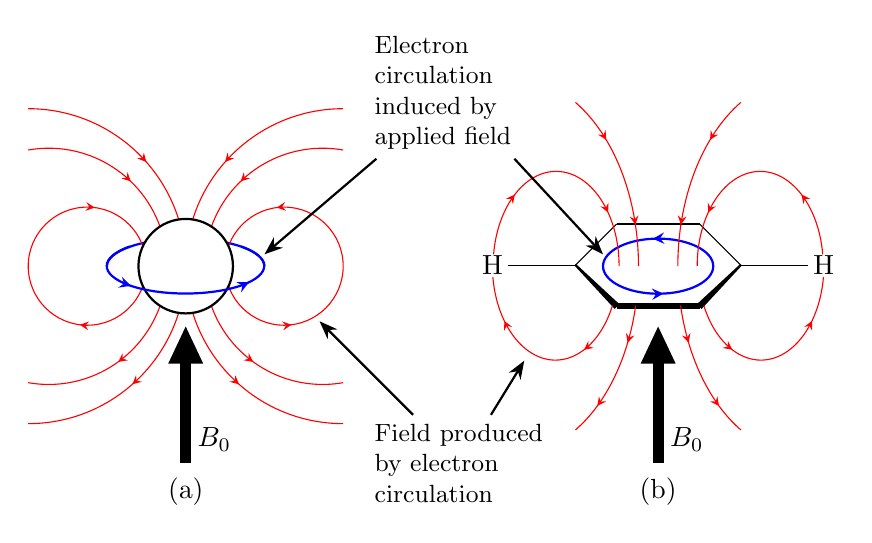
\begin{tikzpicture}[
      decoration={
          markings,
          mark=at position 0.27 with {\arrow{stealth}},
          mark=at position 0.77 with {\arrow{stealth}}
      }
  ]

  %%% Proton shielding
  \begin{scope}[shift={(-3,0)}]
            
      %% Back bond current ring
      \draw [blue, thick] (1,0) arc (0:180:1 and 0.35);
      %% small template ring
      % \draw [gray, postaction={decorate}] (1.3,0) ellipse (0.8 and 1.2);
      %% large template ring
      % \draw [gray, postaction={decorate}] (1.85,0) ellipse (1.6 and 2.4);
      %% Outer field rings
      \draw [red, postaction={decorate}] 
          (2,2) arc (90:270:2);
      \draw [red, postaction={decorate}] 
          (-2,2) arc (90:-90:2);
      
      % \draw [black, postaction={decorate}]
%             (-2.09,0.15) arc (173:0:0.8 and 1.2);
%         \draw [black, postaction={decorate}]
%             (-0.58,-.5) arc (335:187:0.8 and 1.2);
      %% Middle field rings
      % \draw [gray] (0.25,0) arc (-180:180:1.5);
      \draw [red, postaction={decorate}] 
          (2,1.475) arc (80:280:1.5);
      \draw [red, postaction={decorate}] 
          (-2,1.475) arc (100:-100:1.5);
      %% Inner field rings
      \draw [red, postaction={decorate}] 
          (0.5,0) arc (-180:180:0.75);
      \draw [red, postaction={decorate}] 
          (-0.5,0) arc (360:0:0.75);
          
      % Proton
      \draw [black, thick,fill=white] (0,0) circle (0.6);
      
      %% Bond current ring
      \draw [blue, thick, postaction={decorate}] 
          (-.71,.25) arc (135:405:1 and 0.35);
      
      %% External magnetic field
      \draw [black,line width=4pt,arrows={-Triangle[angle=45:15pt]}] 
          (0,-2.5) node[above right=-1pt] {\(B_0\)} node[below] {(a)} -- (0,-0.75);
  \end{scope}
      
  \begin{scope}[shift={(3,0)}]
      %% Benzene molecule
      \node at 
          (0,0) {\chemfig[cram width=2pt]{
              H-?<[7,0.7]-[,,,, line width=2pt]>[1,0.7](-H)-[3,0.7]-[4]?
          }};
      %% Bond current ring
      \draw [blue, thick, postaction={decorate}] 
          (0,0) ellipse (0.7 and 0.35);
      
      %% small template ring
      % \draw [gray, postaction={decorate}] (1.3,0) ellipse (0.8 and 1.2);
      %% large template ring
      % \draw [gray, postaction={decorate}] (1.85,0) ellipse (1.6 and 2.4);
      %% Outer field rings
      \draw [red, postaction={decorate}] 
          (2.09,0.15) arc (7:180:0.8 and 1.2);
      \draw [red, postaction={decorate}] 
          (0.58,-.5) arc (-155:-7:0.8 and 1.2);
      \draw [red, postaction={decorate}] 
          (-2.09,0.15) arc (173:0:0.8 and 1.2);
      \draw [red, postaction={decorate}] 
          (-0.58,-.5) arc (335:187:0.8 and 1.2);
      %% Inner field rings
      \draw [red, postaction={decorate}] 
          (1.05,2.08) arc (120:180:1.6 and 2.4);
      \draw [red, postaction={decorate}] 
          (0.285,-0.50) arc (192:240:1.6 and 2.4);
      \draw [red, postaction={decorate}] 
          (-1.05,2.08) arc (60:0:1.6 and 2.4);
      \draw [red, postaction={decorate}] 
          (-0.285,-0.50) arc (348:300:1.6 and 2.4);
      
      %% External magnetic field
      \draw [black,line width=4pt,arrows={-Triangle[angle=45:15pt]}] 
          (0,-2.5) node[above right=-1pt] {\(B_0\)} node[below] {(b)} -- (0,-0.75);
  \end{scope}
  
  \begin{scope}[node distance=3mm]
      \node[text width=2.2cm,align=left, node font=\small] (a) at (0.5,-2.5) {Field produced by electron\\ circulation};
      \node[text width=2.0cm,align=left, node font=\small] (b) at (0.4,2.2) {Electron\\ circulation\\ induced by\\ applied field};
      
      \draw[-Stealth,thick] (b) -- (-2, 0.15);
      \draw[-Stealth,thick] (b) -- (2.3, 0.15);
      \draw[-Stealth,thick] (a) -- (-1.3, -0.7);
      \draw[-Stealth,thick] (a) -- (1.3, -1.2);

  \end{scope}
\end{tikzpicture}
\setchemfig{atom style={scale=0.80}}

\end{document}

